\documentclass[xelatex,ja=standard,a4paper,9pt]{bxjsarticle}
\usepackage{zxjatype}
\usepackage[haranoaji]{zxjafont}
\usepackage{geometry}
\geometry{margin=14mm}
\usepackage{graphicx,booktabs,xcolor,hyperref,enumitem}
\hypersetup{colorlinks=true,urlcolor=blue!55!black,linkcolor=blue!55!black}
\setlength{\parindent}{0pt}
\setlength{\parskip}{2.5pt}
\setlist{nosep,leftmargin=4mm}
\pagestyle{plain}

\title{\vspace{-12mm}\textbf{EconDID Studio}\\[-1mm]
\large DID・DDD分析を支援する再現可能な研究ソフトウェア}
\author{氏名：\rule{32mm}{0.4pt}\quad 学籍番号：\rule{28mm}{0.4pt}\\
GitHub：\url{https://github.com/panzehui-gh/econ-did-studio}}
\date{2026年8月}

\begin{document}
\maketitle
\vspace{-6mm}

\section*{1. 目的と利用手順}
EconDID Studio は、整理されていない表形式データから差の差法（DID）または
三重差分法（DDD）の推定結果までの反復作業を短縮するソフトウェアである。
利用者は CSV・TSV・Excel を読み込み、基本2×2 DID、個体・時点固定効果 DID、
任意固定効果 DID、DDD のプリセットを選ぶ。ソフトが目的変数、処置、政策後、
個体、時点、第三群の候補を理由と信頼度つきで提示し、利用者は列の意味と二値
変数の向きを確認する。コントロール、固定効果、クラスタを追加して実行すると、
係数表、診断情報、分析対象データ、推定式、statsmodels の全文を保存できる。

因果識別を自動化するものではない。画面には、平行トレンド、先取り行動がない
こと、比較群の妥当性などが因果解釈に別途必要であることを明示した。

\section*{2. 実装上の工夫}
原本を変更しない前処理パイプラインを作り、列名の正規化、欠損表記の統一、空行・
重複行の除去、保守的な数値・日付変換を監査ログに残す。自動列推定はブラック
ボックス分類ではなく、多言語の別名、文字列類似度、型、値の種類数、利用者が
記入した説明を組み合わせた順位付き候補である。未知の二値ラベルを無断で
処置群に割り当てず、必ず向きを確認する。

推定前に DID の4セルまたは DDD の8セル、必要列、二値性、欠損後の標本を検査
する。標準誤差は HC1 または一方向クラスタ頑健を選択できる。希望時のみ、処置群・
対照群の観測平均推移図と、効果推定値・95\%信頼区間・ゼロ線の図を作成する。
DDD の推移図は第三群別の2パネルである。各図は画面表示のほか PNG とベクトル
PDF で出力でき、非専門家向けの平易な解釈文も同時に生成する。

\section*{3. 客観的検証}
検証は二重化した。第一に、既知効果を持つ合成パネルを20シードずつ生成した
モンテカルロ検証では、真の DID 効果2.0に対し平均1.9988、バイアス$-0.0012$、
RMSE 0.0904、95\%区間被覆率0.95、真の DDD 効果1.5に対し平均1.4512、
バイアス$-0.0488$、RMSE 0.1496、被覆率1.00であった。

第二に、通常の一括推定経路とは独立に、NumPy で回帰行列を構成し、擬似逆行列
による OLS と HC1／クラスタ・サンドイッチ分散を手書きした。4プリセットを
各50シード、合計200回照合し、係数・標準誤差とも全件が許容差$10^{-8}$以内で
一致した。係数差の最大値は$1.32\times10^{-14}$、標準誤差差は
$5.38\times10^{-15}$であった。さらに列順序変更、文字列化、四桁丸め、空列、
重複行を含む60回の端から端までの検証を行い、自動役割推定、清掃、推定が全件
成功した（最大推定差$3.09\times10^{-5}$）。

\begin{center}
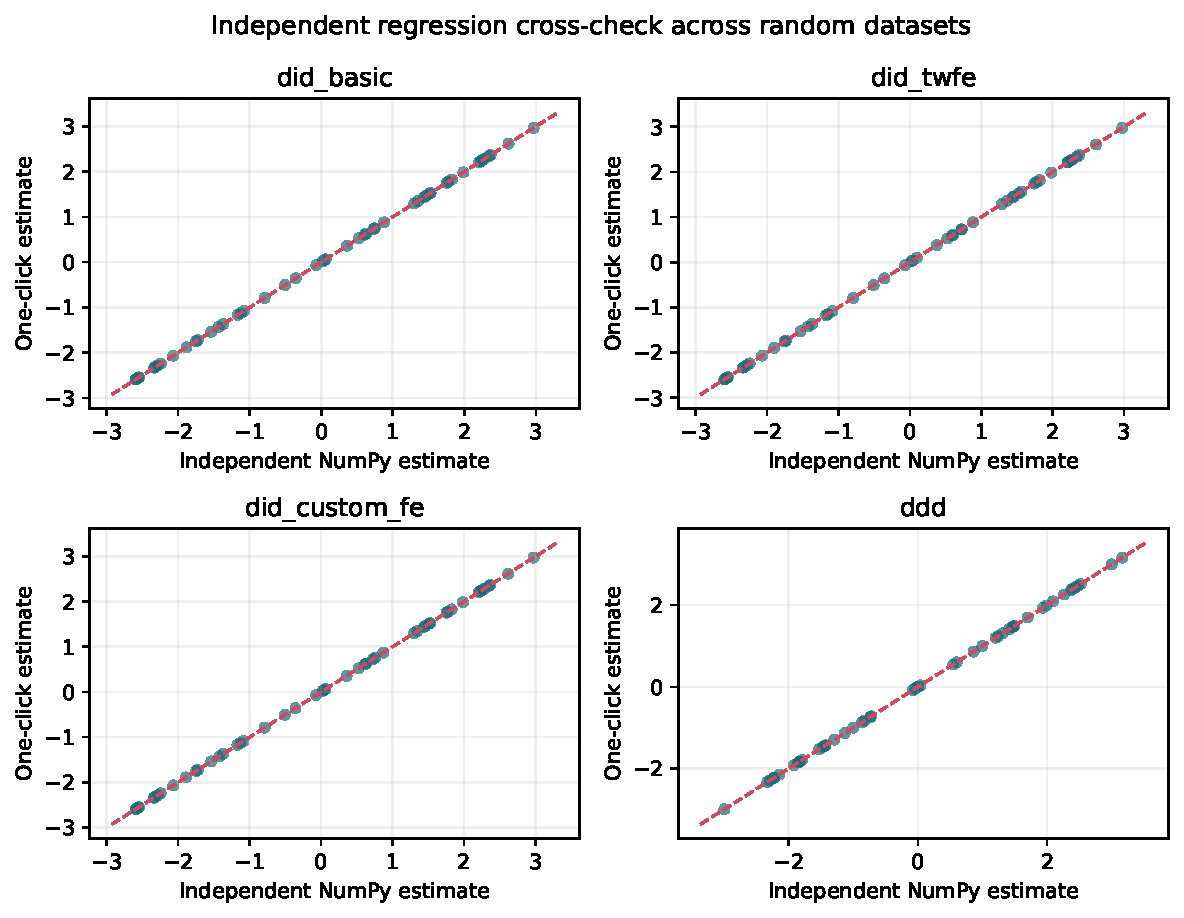
\includegraphics[width=0.77\linewidth]{../docs/cross_validation/manual_vs_one_click.pdf}
\vspace{-2mm}

{\small 図1：独立した NumPy 推定（横軸）と一括推定（縦軸）。破線は完全一致線。}
\end{center}

\section*{4. 再現性・AI利用・制約}
テストは23件あり、GitHub Actions で Python 3.12 上でも実行する構成とした。
依存関係、起動、最短例、開発環境、テスト、検証コマンド、制約を日本語・英語の
README に記載し、MIT License を付与した。OpenAI Codex（GPT-5）を、要件整理、
設計、実装、テスト・文書の草案、失敗原因の診断に利用した。生成物は目視だけで
採用せず、単体テスト、既知効果シミュレーション、独立行列計算で検証した。
現行版は共通の政策開始を示す post 指標を前提とし、段階導入専用推定や
イベントスタディは範囲外である。個人情報・秘密情報を含む実データは収録しない。

\end{document}
